\documentclass[tikz]{standalone}% 'crop' is the default for v1.0, before it was 'preview'
\usepackage{tikz}
\usepackage{pgfplots}
\usepackage{amsmath}

\usepgfplotslibrary{colormaps}
\pgfplotsset{compat=1.18}
\usetikzlibrary{plotmarks, arrows.meta}
%\usetikzlibrary{...}% tikz package already loaded by 'tikz' option
\begin{document}


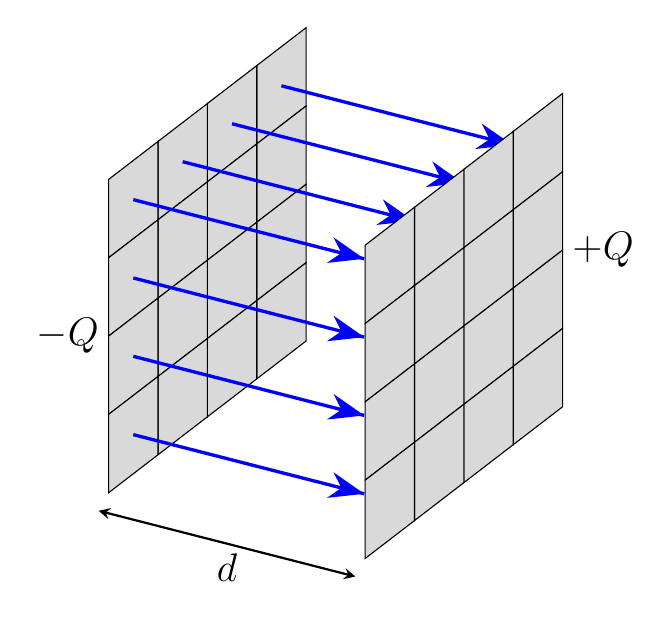
\begin{tikzpicture}[font=\Large]
\begin{axis}[
    hide axis,
    scale=2,
    view={120}{40},
    xmin=-4,xmax=4,
    ymin=-4,ymax=4,
    zmin=-4,zmax=4,
    trig format plots=rad,
  ]
    % Draw first plate
    \addplot3 [ surf, color=gray!30, faceted color=black, domain=-2:2, domain y=-3:3, samples=5, samples y=5]
    ( {x}, 0, {y} );



    % Draw field lines between plates
    \foreach \b in { -2.25, -0.75, 0.75, 2.25 }{%
      \addplot3[samples=2, domain=0:2.7, -{Stealth[scale=1.5]}, blue, very thick, variable=\t] ( 1.5, t, {\b});
    }

    \foreach \a in { -1.5, -0.5, 0.5 }{%
      \addplot3[samples=2, domain=0:2.7, -{Stealth[scale=1.5]}, blue, very thick, variable=\t] ({\a}, t, 2.25);
    }


    % Draw second plate
    \addplot3 [ surf, color=gray!30, faceted color=black, domain=-2:2, domain y=-3:3, samples=5, samples y=5]
    ( {x}, 3, {y} );

    % Add labels
    \node[left] at (2,0,0) {$- Q$};
    \node[right] at (-2,3,0) {$+ Q$};

    % Add arrow
    \draw[stealth-stealth, thick] (2.2,0,-3.2) -- (2.2,3,-3.2) node[midway,below] {$d$};

\end{axis}

\end{tikzpicture}
\end{document}